
\documentclass[12pt]{article}
\usepackage[margin=1in]{geometry}
\usepackage[pdftex]{graphicx}
\usepackage{multirow}
\usepackage{setspace}
\usepackage{enumitem}
\pagestyle{plain}
\setlength\parindent{0pt}

\begin{document}

% Course information
\begin{tabular*}{\textwidth}{l @{\extracolsep{\fill}} r}
  & \multirow{3}{*}{
\includegraphics[height=1.0in]{logo.jpg}} \\
  \large Computers in Physics Exps. & \\
  \large Spring Quarter 2021 & \\
  \large Physics 116C & \\
\end{tabular*}
\vspace{10mm}


% Professor information
\begin{tabular}{ l l }
  \multirow{6}{*}{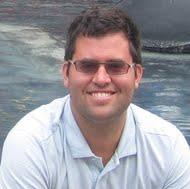
\includegraphics[height=1.25in]{mike.jpg}} & \\
  & \\
  & \large Michael Mulhearn \\
  & \large mulhearn@physics.ucdavis.edu \\
  & \large Physics 317 \\
  & \\
\end{tabular}
\vskip 0.5cm
\noindent
\begin{tabbing}
\hspace*{9em}\= \hspace*{10em} \= \hspace*{6em} \= \kill % set the tabbings
\textbf {Lectures:} \> W  1:10-2:00 PM \> Remote Instruction\\
%\> \> 152 Roessler \> (F) \\
\hspace*{9em}\= \hspace*{5em} \= \hspace*{8em} \= \kill % set the tabbings
\\
\textbf {Labs:}    
\> Section 1: \> M 3:10-6:00 PM \> Remote Instruction \\
\> Section 2: \> W 4:10-7:00 PM \> Remote Instruction \\
\\
\hspace*{9em}\= \kill % set the tabbings
\textbf {References:}  \>  {\tt https://www.scipy-lectures.org} \\
\> Online lecture notes on data analysis and fourier analysis. \\
\textbf{Lab Instructor:} \> TBD \\
\textbf{Final Exam:} \> No Final Exam \\
\end{tabbing}

\noindent
\textbf {Course Description:}
Modern experiments rely heavily on microprocessors to acquire and
analyze experimental data.  We will use Scientific Python for analysis
of experimental data.  Topics include statistical distributions,
experimental uncertainties, statistical analysis, and Fourier
analysis.  We will also study computer architecture and assembly language.\\

\noindent
\textbf {Lectures:}
Lectures will be asynchronous with recorded optional synchronous
recaps and problem-solving sessions.

The optional synchronous lectures will be offered during the Wednesday
lecture slot over zoom.  The lectures will be recorded, but will
include a short unrecorded session for additional questions at the
end.  The recorded lectures will be posted on the course website.

The remaining lecture material will consist of pre-recorded videos
which can be viewed whenever it is convenient.  My experience has been
that pre-recorded videos cover material much faster than traditional
lectures, so generally there will be less than two hours of
pre-recorded content per week.\\

\noindent
\textbf {Labs:}
The lab activities will be asynchronous, but the lab TAs will be
available over zoom to provide help.  Students may attend any lab
section they choose, it does not matter which section you are formally
assigned to.  We may have to revisit this if attendance becomes too
lopsided, but it has worked fine in previous courses.

The due date for each lab will be included with the assignment.  There
is also an automatic one week grace period.  If you are having
difficulty keeping up beyond the grace period, contact the instructor
to devise a schedule.  I am extremely accommodating during remote
learning, but I do not want to encourage procrastination which could
lead to an extremely hectic end of the quarter.\\

\noindent
\textbf {Office Hours:}
The Monday lecture time slot will be repurposed for office hours.
Office hours will not be recorded.  Use the lecture zoom link from the course web site.\\


%\noindent
%\textbf {Lab Safety:}
%Even though you will not be attending lab, you should complete the
%online course for Electrical Safety at \\ {\tt
%  http://safetyservices.ucdavis.edu/training/electrical-safety}\\
%before attempting the Arduino labs.

\noindent
\textbf {Homework:}
There will be five homework assignments, three on statistics, one on
Fourier analysis, and one on assembly.  Using online solution services
is not permitted.  To minimize the effectiveness of online solution
services, homeworks will be graded based on effort only.\\

\noindent
\textbf {Exams:}
There will not be a final exam.  There will be a midterm exam, with format to be determined.\\

\begin{samepage}
\vskip 0.5cm
\noindent
\textbf {Course Outline}:

\begin{table}[h!]
\begin{tabular}{ llll }
\hline
\textbf{Week} & \textbf{Wed Lecture} & \textbf{Lecture} & \textbf{Lab}  \\
\hline
1 & 31 Mar & (No Lecture) & Scipy and Plotting \\
\hline
2 & 7 Apr & Recap S1 & The Monte Carlo Method \\
\hline
3 & 14 Apr & Recap S2 & Limits of Distributions \\
\hline
4 & 21 Apr & Problems &  Uncertainties\\
\hline
5 & 28 Apr & Problems &  Ideal Gas\\
\hline
6 & 5 May & Recap S3  & Curve Fitting \\
\hline 
7 & 12 May & Recap S3  & (catchup) \\
% F: 
\hline
8 & 19 May & Fourier & TBD \\
\hline
9 & 26 May & Problems & TBD \\
% F: 
\hline
10 & 2 Jun & Problems  & No Lab \\
% F: 
\hline
\end{tabular} 
\end{table}
\end{samepage}
\end{document}

